\chapter{Artificial Neural Network (ANN)}

\section{Perceptron \cite{wiki-perceptron}}\label{perceptron}

\begin{figure}[H]
    \centering
    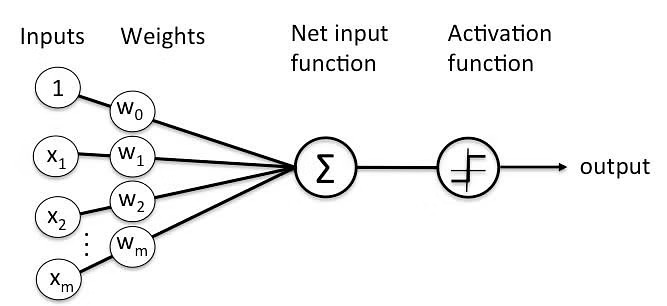
\includegraphics[height=3cm]{Pictures/deep_neural_networks/perceptron.jpg}
    \caption{Perceptron}
\end{figure}

In machine learning, the perceptron (or McCulloch–Pitts neuron) is an algorithm for supervised learning of binary classifiers. A binary classifier is a function which can decide whether or not an input, represented by a vector of numbers, belongs to some specific class. It is a type of linear classifier, i.e. a classification algorithm that makes its predictions based on a linear predictor function combining a set of weights with the feature vector.


\section{Artificial neuron \cite{wiki-Artificial_neuron}}\label{Artificial neuron}
\begin{table}[H]
    \begin{minipage}{0.45\textwidth}
        \begin{figure}[H]
            \centering
            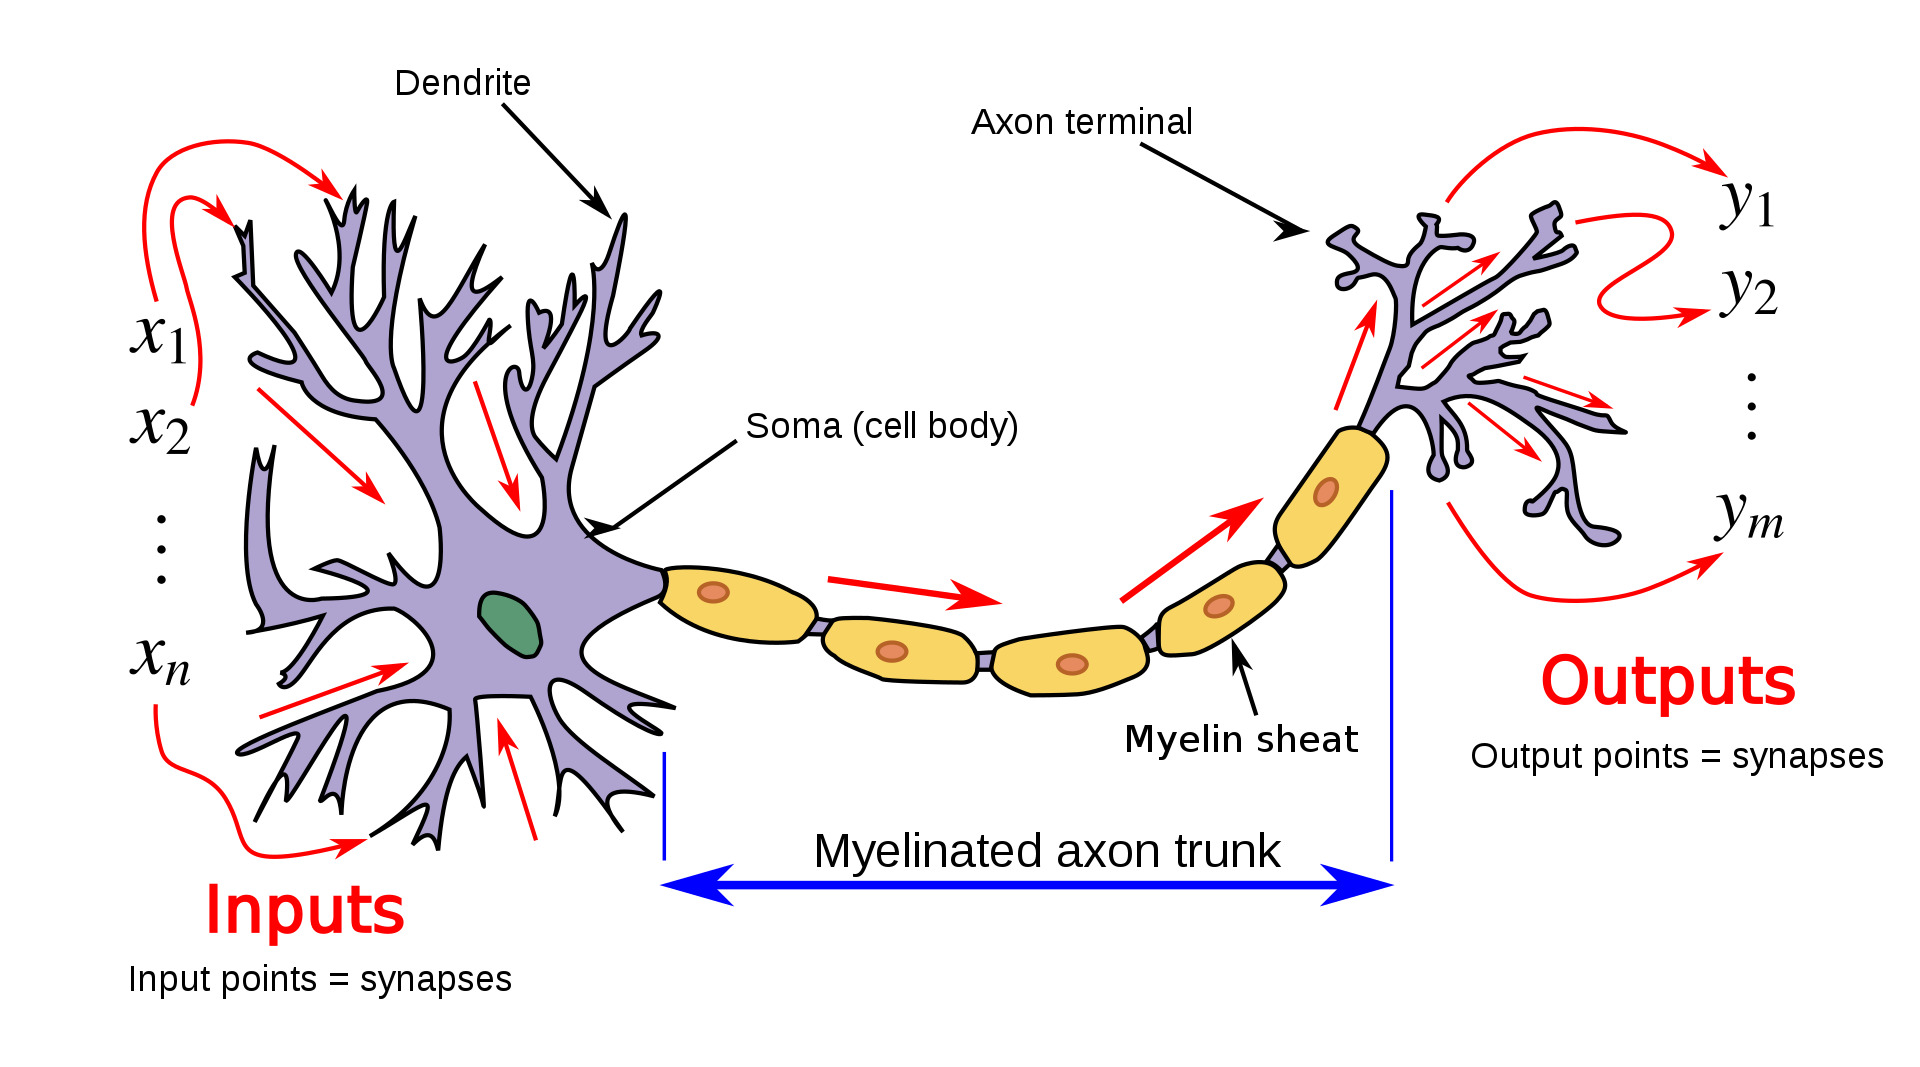
\includegraphics[height=4cm]{Pictures/deep_neural_networks/bio_neuron.jpg}
            \caption{ANN: Biological Neuron}
        \end{figure}
    \end{minipage}
    \hfill
    \begin{minipage}{0.45\textwidth}
        \begin{figure}[H]
            \centering
            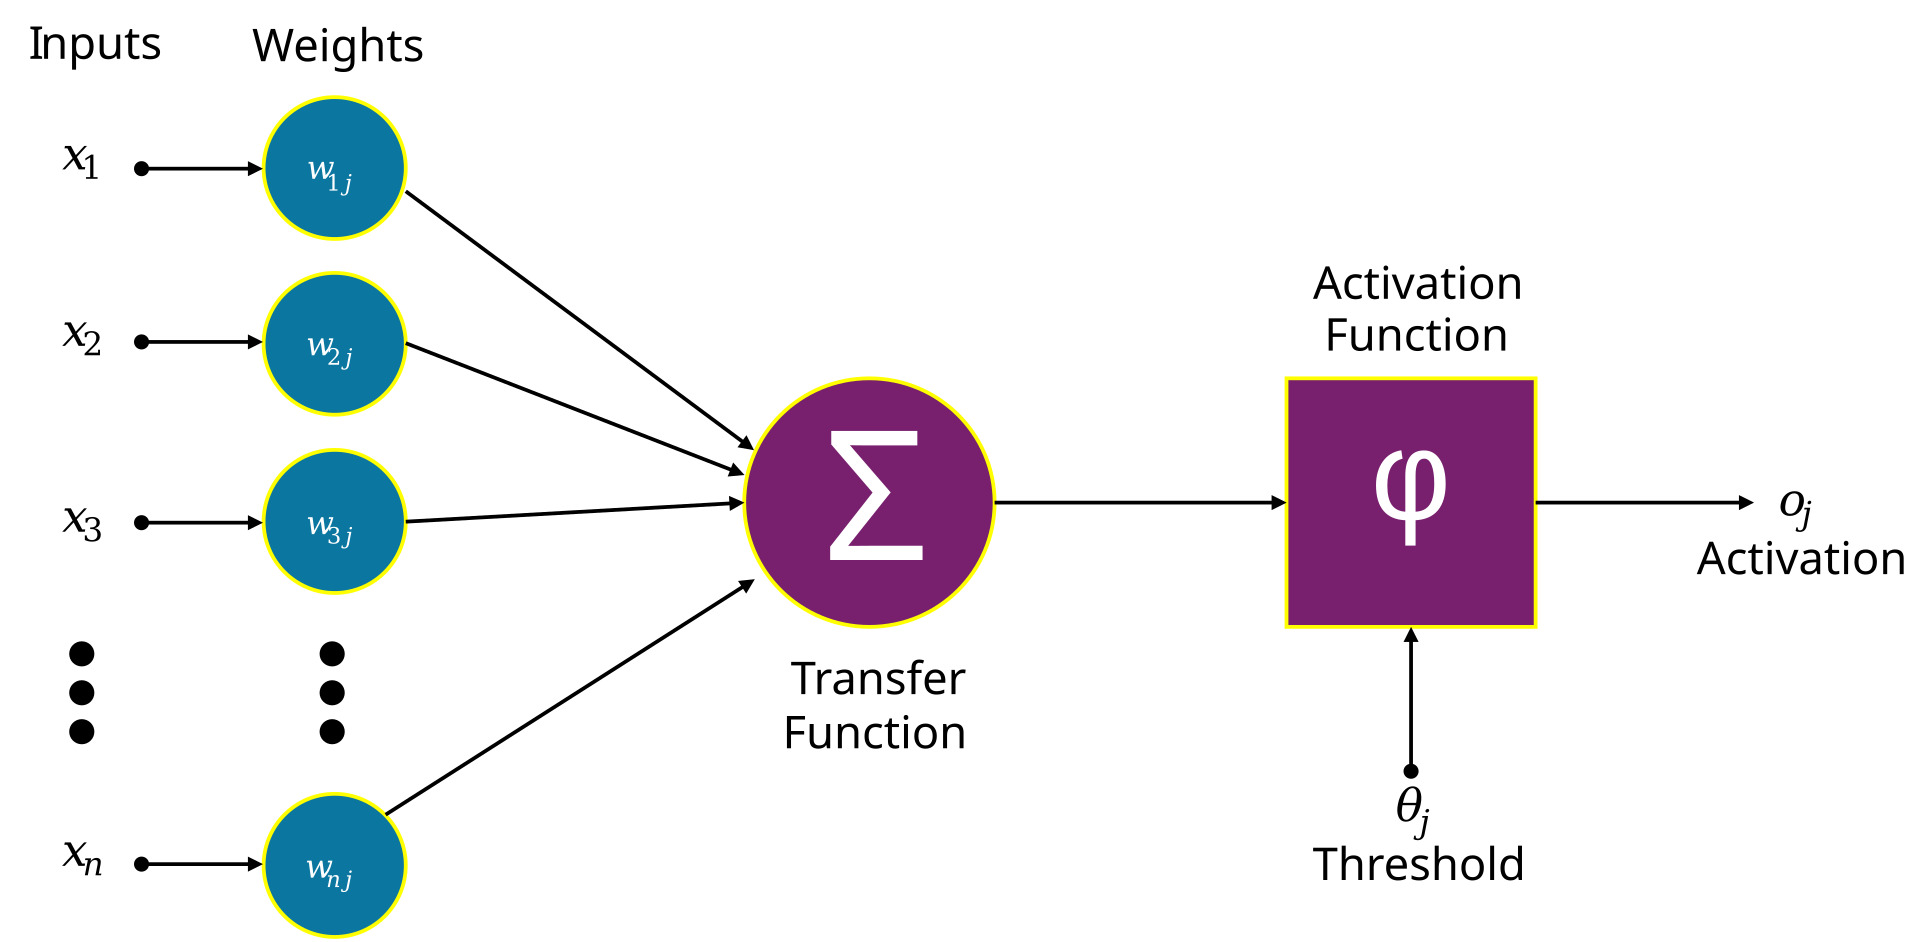
\includegraphics[height=4cm]{Pictures/deep_neural_networks/Artificial_neuron_structure.jpg}
            \caption{ANN: Artificial Neuron}
        \end{figure}
    \end{minipage}
\end{table}


An artificial neuron is a mathematical function conceived as a model of biological neurons in a neural network. Artificial neurons are the elementary units of artificial neural networks. The artificial neuron is a function that receives one or more inputs, applies weights to these inputs, and sums them to produce an output.


Usually, each input is separately weighted, and the sum is often added to a term known as a bias (loosely corresponding to the threshold potential), before being passed through a non-linear function known as an \textbf{activation function} or \textbf{transfer function}.

\[
     y_{k}=\varphi \left(\sum _{j=0}^{m}w_{kj}x_{j}\right)
\]


SEE: \fullref{Perceptron vs Artificial Neuron}



\section{Activation Function \cite{wiki-Artificial_neuron, wiki-activation-fn}}
The activation function of a node in an artificial neural network is a function that calculates the output of the node based on its individual inputs and their weights. Nontrivial problems can be solved using only a few nodes if the activation function is nonlinear


\begin{enumerate}
    \item  The transfer functions usually have a \textbf{sigmoid} shape, but they may also take the form of other non-linear functions, piecewise linear functions, or step functions.
    \item They are also often monotonically increasing, continuous, differentiable and bounded. 
    \item  Non-monotonic, unbounded and oscillating activation functions with multiple zeros that outperform sigmoidal and ReLU-like activation functions on many tasks have also been recently explored
\end{enumerate}

See \ref{chapter: Activation Functions} for more details.





\section{Moving towards multi layer models}
\subsection{Limitations of Linear Models \cite{dnn-1}}

\begin{enumerate}
    \item linearity implies the \textbf{weaker assumption of monotonicity}, i.e., that any increase in our feature must either always cause an increase in our model’s output (if the corresponding weight is positive), or always cause a decrease in our model’s output (if the corresponding weight is negative).

    \item We can overcome the limitations of linear models by incorporating one or more hidden layers

    \item The easiest way to do this is to stack many fully connected layers on top of one another. Each layer feeds into the layer above it, until we generate outputs. 
\end{enumerate}

\subsection{From Linear to Nonlinear \cite{dnn-1}}

\begin{customTableWrapper}{1.5}
\begin{table}[H]
    \centering
    \begin{tabular}{|l|p{9cm}|}
        \hline
        \customTableHeaderColor
        \multicolumn{2}{|c|}{Input layer} \\ \hline
    
        $n$ & num of examples in a \textbf{minibatch} \\
        $d$ & num of inputs/ features \\
        $\mathbf{X} \in \mathbb{R}^{n \times d}$ & examples in a \textbf{minibatch} \\

        \hline
        \customTableHeaderColor
        \multicolumn{2}{|c|}{Hidden layer} \\ \hline
        
        $h$ & num of hidden units in a hidden layer \\
        $\mathbf{W}^{(1)} \in \mathbb{R}^{d \times h}$ & weights \\
        $\mathbf{b}^{(1)} \in \mathbb{R}^{1 \times h}$ & biases \\
        $\sigma$ & \textbf{nonlinear} activation function \\
        $\mathbf{H} \in \mathbb{R}^{n \times h}$ & outputs of the hidden layer, which are \textbf{hidden representations} \indexlabel{hidden representations}\\

        \hline
        \customTableHeaderColor
        \multicolumn{2}{|c|}{Output Layer} \\ \hline

        $\mathbf{W}^{(2)} \in \mathbb{R}^{h \times q}$ & weights \\
        $\mathbf{b}^{(2)} \in \mathbb{R}^{1 \times q}$ & biases \\
        $\mathbf{O} \in \mathbb{R}^{n \times q}$ & output of output layer \\
        
        \hline
    \end{tabular}
\end{table}
\end{customTableWrapper}

\begin{enumerate}
    \item input layer has no weights, biases or outputs

    \item $
        \hfill
        \mathbf{H} = \sigma(\mathbf{X} \mathbf{W}^{(1)} + \mathbf{b}^{(1)})
        \hfill
        \mathbf{O} = \mathbf{H}\mathbf{W}^{(2)} + \mathbf{b}^{(2)}
        \hfill
    $

    

\end{enumerate}


\section{Connectionism model \cite{wiki-Connectionism}}\label{Connectionism model}
Connectionism (coined by Edward Thorndike in the 1931) is the name of an approach to the study of human mental processes and cognition that utilizes mathematical models known as connectionist networks or artificial neural networks. Connectionism has had many 'waves' since its beginnings.

\section{Artificial Neural Network (ANN) \cite{wiki-ann}}\label{ann}
\begin{figure}[H]
    \centering
    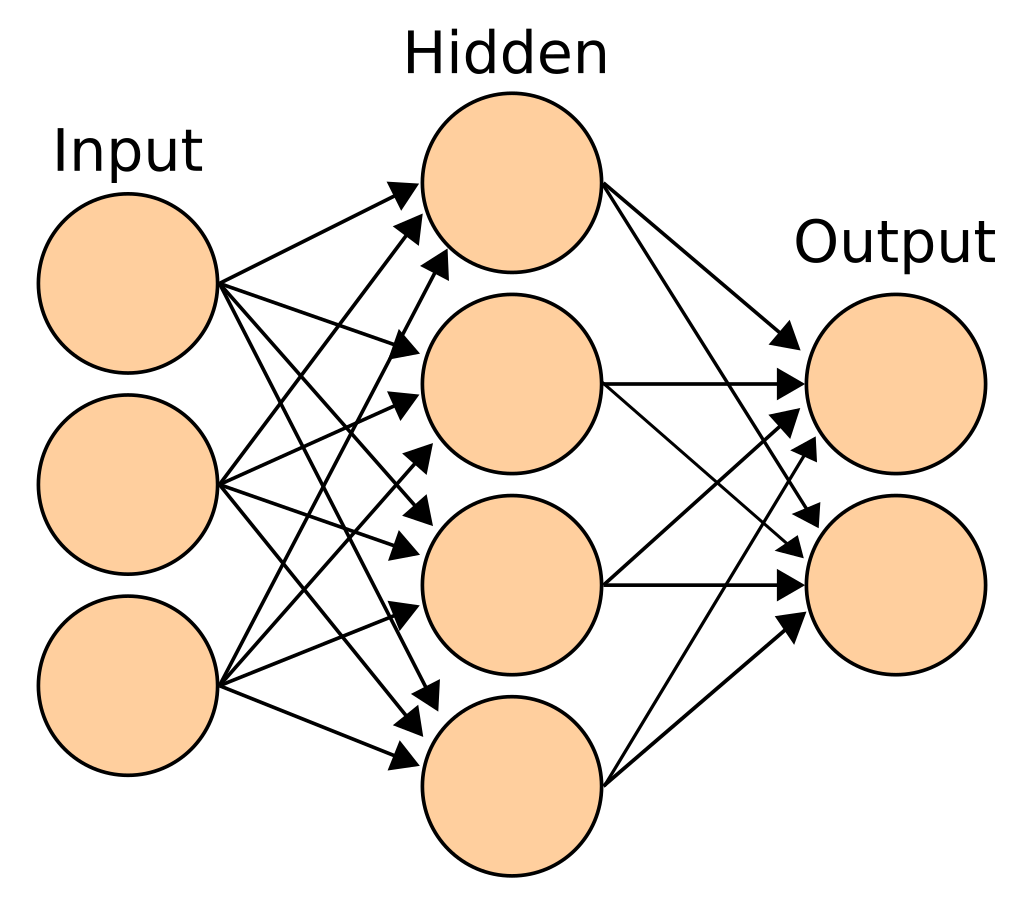
\includegraphics[height=4cm]{Pictures/deep_neural_networks/ann.png}
    \caption{Artificial Neural Network}
\end{figure}
A neural network (also artificial neural network or neural net, abbreviated ANN or NN) is a model inspired by the structure and function of biological neural networks in animal brains. An ANN consists of connected units or nodes called \textbf{artificial neurons}, which loosely model the neurons in a brain. These are connected by edges, which model the synapses in a brain. Each artificial neuron receives signals from connected neurons, then processes them and sends a signal to other connected neurons. The "signal" is a real number, and the output of each neuron is computed by some non-linear function of the sum of its inputs, called the \textbf{activation function}. The strength of the signal at each connection is determined by a weight, which adjusts during the learning process.

SEE: \fullref{connectionism vs ann}

\begin{enumerate}
    \item ANN is subset of Connectionism
\end{enumerate}


\section{Perceptron Learning Algorithm \cite{medium-perceptron-learning-algorithm}}\label{Perceptron Learning Algorithm}

\begin{enumerate}
    \item Goal is to find the w vector that can perfectly classify positive inputs and negative inputs in the data.
\end{enumerate}

\begin{algorithm}[H]
    \caption{Perceptron Learning Algorithm}
    $P \gets$ inputs with label 1\;
    $N \gets$ inputs with label 0\;
    Initialize $\textbf{w}$ randomly\;
    \While{!convergence}{
        Pick random $x \in P \cup N$\;
        \If{$x \in P$ and $w \cdot x < 0$}{
            $w = w + x$\;
        }
        \If{$x \in N$ and $w \cdot x \ge 0$}{
            $w = w - x$\;
        }
    }
\end{algorithm}

Examples:\\
\begin{enumerate}
    \item \url{https://www.geeksforgeeks.org/implementation-of-perceptron-algorithm-for-or-logic-gate-with-2-bit-binary-input/}
    \item \url{https://www.geeksforgeeks.org/implementation-of-perceptron-algorithm-for-and-logic-gate-with-2-bit-binary-input/}
    \item \url{https://www.geeksforgeeks.org/implementation-of-perceptron-algorithm-for-not-logic-gate/}
    \item \url{https://turcomat.org/index.php/turkbilmat/article/view/7786}
\end{enumerate}



\section{Multilayer Perceptron (MLP) \cite{wiki-Multilayer_perceptron,dnn-1}} \label{Multilayer_perceptron}

\begin{enumerate}
    \item The \textbf{simplest} deep networks are called multilayer perceptrons.

    \item MLP is a specific type of ANN, meaning all MLPs are ANNs, but not all ANNs are MLPs.
    
    \item A multilayer perceptron (MLP) is a name for a modern feedforward artificial neural network, consisting of \textbf{fully connected neurons} with a nonlinear activation function, organized in at least three layers, notable for being able to distinguish data that is not linearly separable.

    \item Modern feedforward networks are trained using the backpropagation method and are colloquially referred to as the "vanilla" neural networks.

    \item MLPs grew out of an effort to improve single-layer perceptrons, which could only distinguish linearly separable data. 

    \item A perceptron traditionally used a Heaviside step function as its nonlinear activation function. 
    
    \item However, the backpropagation algorithm requires that modern MLPs use continuous activation functions such as sigmoid or ReLU.

    
\end{enumerate}


\noindent
\textbf{SEE}: \fullref{mlp vs ann}



\section{NN as \textit{Universal Approximators} \cite{dnn-1}} \label{nn as Universal Approximators}

\begin{enumerate}
    \item even with a single-hidden-layer network, given enough nodes (possibly absurdly many), and the right set of weights, we can model any function.

    \item Moreover, just because a single-hidden-layer network can learn any function does not mean that you should try to solve all of your problems with one. In fact, in this case kernel methods are way more effective, since they are capable of solving the problem exactly even in infinite dimensional spaces.

\end{enumerate}


\section{Forward Propagation/ forward pass \cite{dnn-1}} \label{Forward Propagation/ forward pass}


\begin{enumerate}[itemsep=0.1cm]
    \item Forward propagation (or forward pass) refers to the calculation and storage of intermediate variables (including outputs) for a neural network in order from the input layer to the output layer.

\end{enumerate}


\textbf{Example}: \\


\textbf{Assumptions}:
\begin{enumerate}
    \item hidden layer does not include a bias term
    \item output layer possess only a weight
\end{enumerate}

\begin{customTableWrapper}{1.5}
\begin{table}[H]
    \centering
    \begin{tabular}{|l|p{8cm}|}
        \hline

        \customTableHeaderColor
        \multicolumn{2}{|c|}{Input Layer} \\ \hline
        
        $\mathbf{x}\in \mathbb{R}^d$ & input example \\
        $y$ & example label \\

        \hline
        \customTableHeaderColor
        \multicolumn{2}{|c|}{Hidden Layer} \\ \hline
        
        $h$ & number of hidden units \\
        $\mathbf{W}^{(1)} \in \mathbb{R}^{h \times d}$ & weight parameter \\ 
        $\mathbf{z}= \mathbf{W}^{(1)} \mathbf{x} \in \mathbb{R}^h$ & intermediate variable \\
        $\phi$ & activation function \\
        $\mathbf{h}= \phi (\mathbf{z})$ & hidden activation vector \\

        \hline
        \customTableHeaderColor
        \multicolumn{2}{|c|}{Output Layer} \\ \hline
        
        $q$ & number of output units \\
        $\mathbf{W}^{(2)} \in \mathbb{R}^{q \times h}$ & weights \\
        $\mathbf{o}= \mathbf{W}^{(2)} \mathbf{h}$ & output layer variable \\

        \hline
        \customTableHeaderColor
        \multicolumn{2}{|c|}{After Output Layer} \\ \hline

        $l$ & loss function \\
        
        $L = l(\mathbf{o}, y)$ & loss term for a single data example \\
        
        $\lambda$ & hyperparameter for $l_2$ regularization \\
        
        $s = \dfrac{\lambda}{2} \left(\|\mathbf{W}^{(1)}\|_\textrm{F}^2 + \|\mathbf{W}^{(2)}\|_\textrm{F}^2\right)$ & regularization term \\[1ex]

        $J = L + s$ & model’s regularized loss on a given data example (aka \textbf{objective function}) \\

        \hline
    \end{tabular}
\end{table}
\end{customTableWrapper}

\begin{enumerate}
    \item The hidden layer output $\mathbf{h}$ is also an intermediate variable.
\end{enumerate}

\subsection{Computational Graph of Forward Propagation \cite{dnn-1}}

\begin{figure}[H]
    \centering
    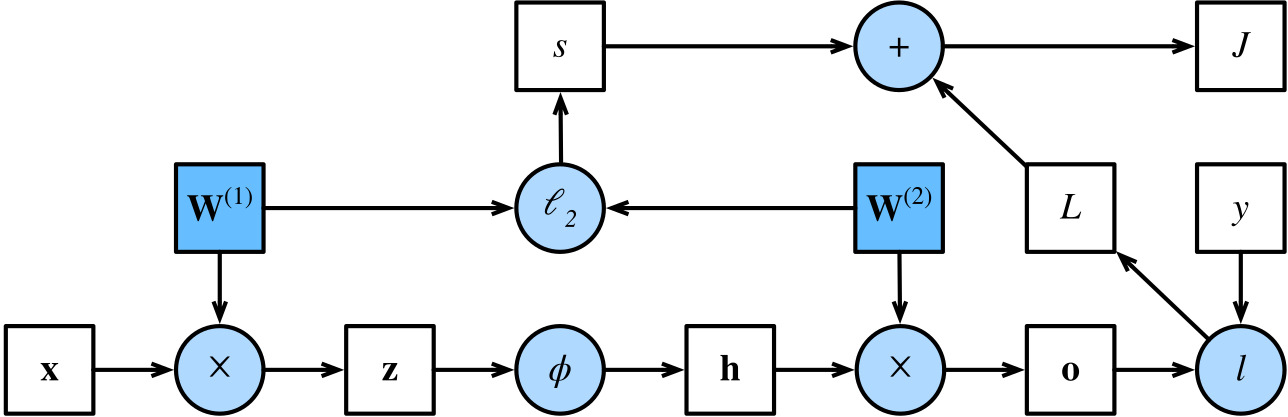
\includegraphics[width=\linewidth, height=3cm, keepaspectratio]{Pictures/deep_neural_networks/Computational Graph of Forward Propagation-5.3.1.jpg}
\end{figure}

\begin{enumerate}
    \item Plotting computational graphs helps us visualize the dependencies of operators and variables within the calculation.

    \item squares denote variables
    \item circles denote operators 
    
    \item The lower-left corner signifies the input and the upper-right corner is the output. 
    
    \item The directions of the arrows (which illustrate data flow) are primarily rightward and upward.

\end{enumerate}




\section{Backpropagation \cite{dnn-1}} \label{Backpropagation}

\begin{enumerate}[itemsep=0.2cm]
    \item Backpropagation refers to the method of calculating the gradient of neural network parameters.

    \item the method traverses the network in \textbf{reverse order}, from the output to the input layer, according to the \textbf{chain rule} from calculus. 
    
    \item The algorithm stores any intermediate variables (\textbf{partial derivatives}) required while calculating the gradient with respect to some parameters.

    \item[] 
    $
        \dfrac{\partial J}{\partial L} = 1
        \hfill
        \dfrac{\partial J}{\partial s} = 1
        \hfill
        \dfrac{\partial J}{\partial \mathbf{o}}
        = \dfrac{\partial J}{\partial L}\dfrac{\partial L}{\partial \mathbf{o}}
        = \dfrac{\partial L}{\partial \mathbf{o}}
        \in \mathbb{R}^q
        \hfill
        \dfrac{\partial s}{\partial \mathbf{W}^{(1)}} = \lambda \mathbf{W}^{(1)}
        \hfill
        \dfrac{\partial s}{\partial \mathbf{W}^{(2)}} = \lambda \mathbf{W}^{(2)}
    $

    \item[] 
    $
        \dfrac{\partial J}{\partial \mathbf{W}^{(2)}}
        = \dfrac{\partial J}{\partial \mathbf{o}}\dfrac{\partial \mathbf{o}}{\partial \mathbf{W}^{(2)}}
        + \dfrac{\partial J}{\partial s}, \dfrac{\partial s}{\partial \mathbf{W}^{(2)}}
        = \dfrac{\partial J}{\partial \mathbf{o}} \mathbf{h}^\top + \lambda \mathbf{W}^{(2)}
        \hfill
        \dfrac{\partial J}{\partial \mathbf{h}}
        = \dfrac{\partial J}{\partial \mathbf{o}} \dfrac{\partial \mathbf{o}}{\partial \mathbf{h}}
        = {\mathbf{W}^{(2)}}^\top \dfrac{\partial J}{\partial \mathbf{o}}
    $

    \item[] 
    $
        \dfrac{\partial J}{\partial \mathbf{z}}
        = \dfrac{\partial J}{\partial \mathbf{h}} \dfrac{\partial \mathbf{h}}{\partial \mathbf{z}}
        = \dfrac{\partial J}{\partial \mathbf{h}} \odot \phi'\left(\mathbf{z}\right)
        \hfill
        \dfrac{\partial J}{\partial \mathbf{W}^{(1)}}
        = \dfrac{\partial J}{\partial \mathbf{z}} \dfrac{\partial \mathbf{z}}{\partial \mathbf{W}^{(1)}}
        + \dfrac{\partial J}{\partial s} \dfrac{\partial s}{\partial \mathbf{W}^{(1)}}
        = \dfrac{\partial J}{\partial \mathbf{z}} \mathbf{x}^\top + \lambda \mathbf{W}^{(1)}
    $

    \item Since the activation function $\phi$ applies elementwise, calculating the gradient $\partial J/\partial \mathbf{z} \in \mathbb{R}^h$ of the intermediate variable $\mathbf{z}$ requires that we use the elementwise multiplication operator, which we denote by $\odot$.

    
\end{enumerate}


\section{Training Neural Networks \cite{dnn-1}}

\begin{enumerate}
    \item When training neural networks, forward and backward propagation depend on each other. 
    
    \item For forward propagation, we traverse the computational graph in the direction of dependencies and compute all the variables on its path. 
    
    \item These are then used for backpropagation where the compute order on the graph is reversed.

    \item On the one hand, computing the regularization term during forward propagation depends on the current values of model parameters $\mathbf{W}^{(1)}$ and $\mathbf{W}^{(2)}$.\\
    They are given by the optimization algorithm according to backpropagation in the most recent iteration.\\
    On the other hand, the gradient calculation for the parameter during backpropagation depends on the current value of the hidden layer output $\mathbf{h}$, which is given by forward propagation.


\end{enumerate}


\section{Vanishing and Exploding Gradients \cite{dnn-1}} \label{Vanishing and Exploding Gradients}

\begin{customTableWrapper}{1.5}
\begin{table}[H]
    \centering
    \begin{tabular}{|l|p{8cm}|}
        \hline
        
        $L$ & Num of layers \\

        $\mathbf{x}$ & input \\

        $\mathbf{o}$ & output \\

        $l$ & layer \\

        $f_l$ & transformation \\

        $\mathbf{W}^{(l)}$ & transformation parameters \\

        $\mathbf{h}^{(l)}$ & hidden layer output ($\mathbf{h}^{(0)} = \mathbf{x}$) \\

        
        
        \hline
    \end{tabular}
\end{table}
\end{customTableWrapper}

\begin{enumerate}[itemsep=0.2cm]
    \item network:
    $
        \hfill
        \mathbf{h}^{(l)} = f_l (\mathbf{h}^{(l-1)})
        \hfill
        \mathbf{o} = f_L \circ \cdots \circ f_1(\mathbf{x}).
        \hfill
    $

    \item[] 
    $
        \hfill
        \partial_{\mathbf{W}^{(l)}} \mathbf{o} 
        = \underbrace{\partial_{\mathbf{h}^{(L-1)}} \mathbf{h}^{(L)}}_{ \mathbf{M}^{(L)} \stackrel{\textrm{def}}{=}} 
        \cdots 
        \underbrace{\partial_{\mathbf{h}^{(l)}} \mathbf{h}^{(l+1)}}_{ \mathbf{M}^{(l+1)} \stackrel{\textrm{def}}{=}} 
        \underbrace{\partial_{\mathbf{W}^{(l)}} \mathbf{h}^{(l)}}_{ \mathbf{v}^{(l)} \stackrel{\textrm{def}}{=}}
        \hfill
    $
    
    \item gradient is the product of $L-l$ matrices $\mathbf{M}^{(L)} \cdots \mathbf{M}^{(l+1)}$ and the gradient vector $\mathbf{v}^{(l)}$.

    \item we are susceptible to the same problems of \textbf{numerical underflow} that often crop up when multiplying together too many probabilities. 
    
    \item When dealing with probabilities, a common trick is to switch into log-space, i.e., shifting pressure from the mantissa to the exponent of the numerical representation. 
    
    \item Unfortunately, our problem above is more serious: initially the matrices $\mathbf{M}^{(l)}$ may have a wide variety of eigenvalues. \\
    They might be small or large, and their product might be very large or very small.

    \item The risks posed by unstable gradients go beyond numerical representation. Gradients of unpredictable magnitude also threaten the stability of our optimization algorithms. We may be facing parameter updates that are either
    \begin{enumerate}
        \item excessively large, destroying our model (the exploding gradient problem) 
        
        \item  excessively small (the vanishing gradient problem)

    \end{enumerate}
    rendering learning impossible as parameters hardly move on each update.

    \item \textbf{Vanishing Gradient}: When our network boasts many layers, unless we are careful, the gradient will likely be cut off at some layer. Indeed, this problem used to plague deep network training. Consequently, ReLUs, which are more stable (but less neurally plausible), have emerged as the default choice for practitioners.

    \item \textbf{Exploding Gradient}: When this happens because of the initialization of a deep network, we have no chance of getting a gradient descent optimizer to converge.

\end{enumerate}


\section{Parameter Initialization \cite{dnn-1}} \label{Parameter Initialization}

\subsection{Default Initialization \cite{dnn-1}} \label{Parameter Initialization: Default Initialization}

\begin{enumerate}
    \item we use a normal distribution to initialize the values of our weights. 
    
    \item If we do not specify the initialization method, the framework will use a default random initialization method, which often works well in practice for moderate problem sizes.

\end{enumerate}


\subsection{Xavier Initialization \cite{dnn-1}} \label{Parameter Initialization: Xavier Initialization}

\begin{customTableWrapper}{1.5}
\begin{table}[H]
    \centering
    \begin{tabular}{l p{8cm}}
        $n_\textrm{in}$ & number of inputs \\

        $x_j$ & inputs \\

        $w_{ij}$ & weights \\
        
        $o_{i} = \dsum_{j=1}^{n_\textrm{in}} w_{ij} x_j$ & output for some fully connected layer without nonlinearities. \\[1ex]

        $n_\textrm{out}$ & number of outputs \\
    \end{tabular}
\end{table}
\end{customTableWrapper}

\begin{enumerate}[itemsep=0.2cm]
    \item The weights $w_{ij}$ are all drawn independently from the same distribution.
    
    \item let’s assume that this distribution has zero mean and variance $\sigma^2$.
    
    \item this does \textbf{NOT} mean that the distribution has to be Gaussian, just that the mean and variance need to exist.

    \item let’s assume that the inputs to the layer $x_j$ also have zero mean and variance $\gamma^2$ and that they are independent of $w_{ij}$ and independent of each other.

    \item[] 
    $
        \hfill
        E[o_i] 
        = \dsum_{j=1}^{n_\textrm{in}} E[w_{ij} x_j]
        = \dsum_{j=1}^{n_\textrm{in}} E[w_{ij}] E[x_j]
        = 0 
        \hfill
    $

    \item[] 
    $
        \hfill
        \textrm{Var}[o_i] 
        = E[o_i^2] - (E[o_i])^2
        = \dsum_{j=1}^{n_\textrm{in}} E[w^2_{ij} x^2_j] - 0
        = \dsum_{j=1}^{n_\textrm{in}} E[w^2_{ij}] E[x^2_j] 
        = n_\textrm{in} \sigma^2 \gamma^2
        \hfill
    $

    \item One way to keep the variance fixed is to set $n_\textrm{in} \sigma^2 = 1$. \\
    Using the same reasoning as for forward propagation, we see that the gradients’ variance can blow up unless $n_\textrm{out} \sigma^2 = 1$
    \[
        \hfill
        \dfrac{1}{2} (n_\textrm{in} + n_\textrm{out}) \sigma^2 = 1 
        \hspace{0.5cm}
        \Rightarrow
        \sigma = \sqrt{\dfrac{2}{n_\textrm{in} + n_\textrm{out}}}
        \hfill
    \]

    \item This is the reasoning underlying the now-standard and practically beneficial Xavier initialization\\
    Xavier initialization samples weights from a Gaussian distribution with zero mean and variance $\sigma^2 = \frac{2}{n_\textrm{in} + n_\textrm{out}}$

    \item We can also adapt this to choose the variance when sampling weights from a uniform distribution. Note that the uniform distribution $U(-a, a)$ has variance $\dfrac{a^2}{3}$.
    \[
        \hfill
        U\dParenBrac{
            -\sqrt{\dfrac{6}{n_\textrm{in} + n_\textrm{out}}}, 
            \sqrt{\dfrac{6}{n_\textrm{in} + n_\textrm{out}}}
        }
        \hfill
    \]
\end{enumerate}



\section{Layers and modules \cite{dnn-1}}

\begin{enumerate}
    \item For MLPs, both the entire model and its constituent layers share this structure:\\
    The \textbf{entire model} takes in raw \textbf{inputs} (the features), generates \textbf{outputs} (the predictions), and possesses \textbf{parameters} (the combined parameters from all constituent layers).\\
    Likewise, each \textbf{individual layer} ingests \textbf{inputs} (supplied by the previous layer) generates \textbf{outputs} (the inputs to the subsequent layer), and possesses a set of \textbf{tunable parameters} that are updated according to the signal that flows backwards from the subsequent layer.

    \item A \textbf{module} \indexlabel{module} could describe a single layer, a component consisting of multiple layers, or the entire model itself.

    
\end{enumerate}


\section{Parameter Management \cite{dnn-1}}

\begin{enumerate}[itemsep=0.2cm]
    \item Parameter Access
    \begin{enumerate}
        \item Each layer’s parameters are conveniently located in its attribute.

    \end{enumerate}

\end{enumerate}



\section{Function Classes \cite{dnn-1}} \label{nn: Function Classes}

\begin{figure}[H]
    \centering
    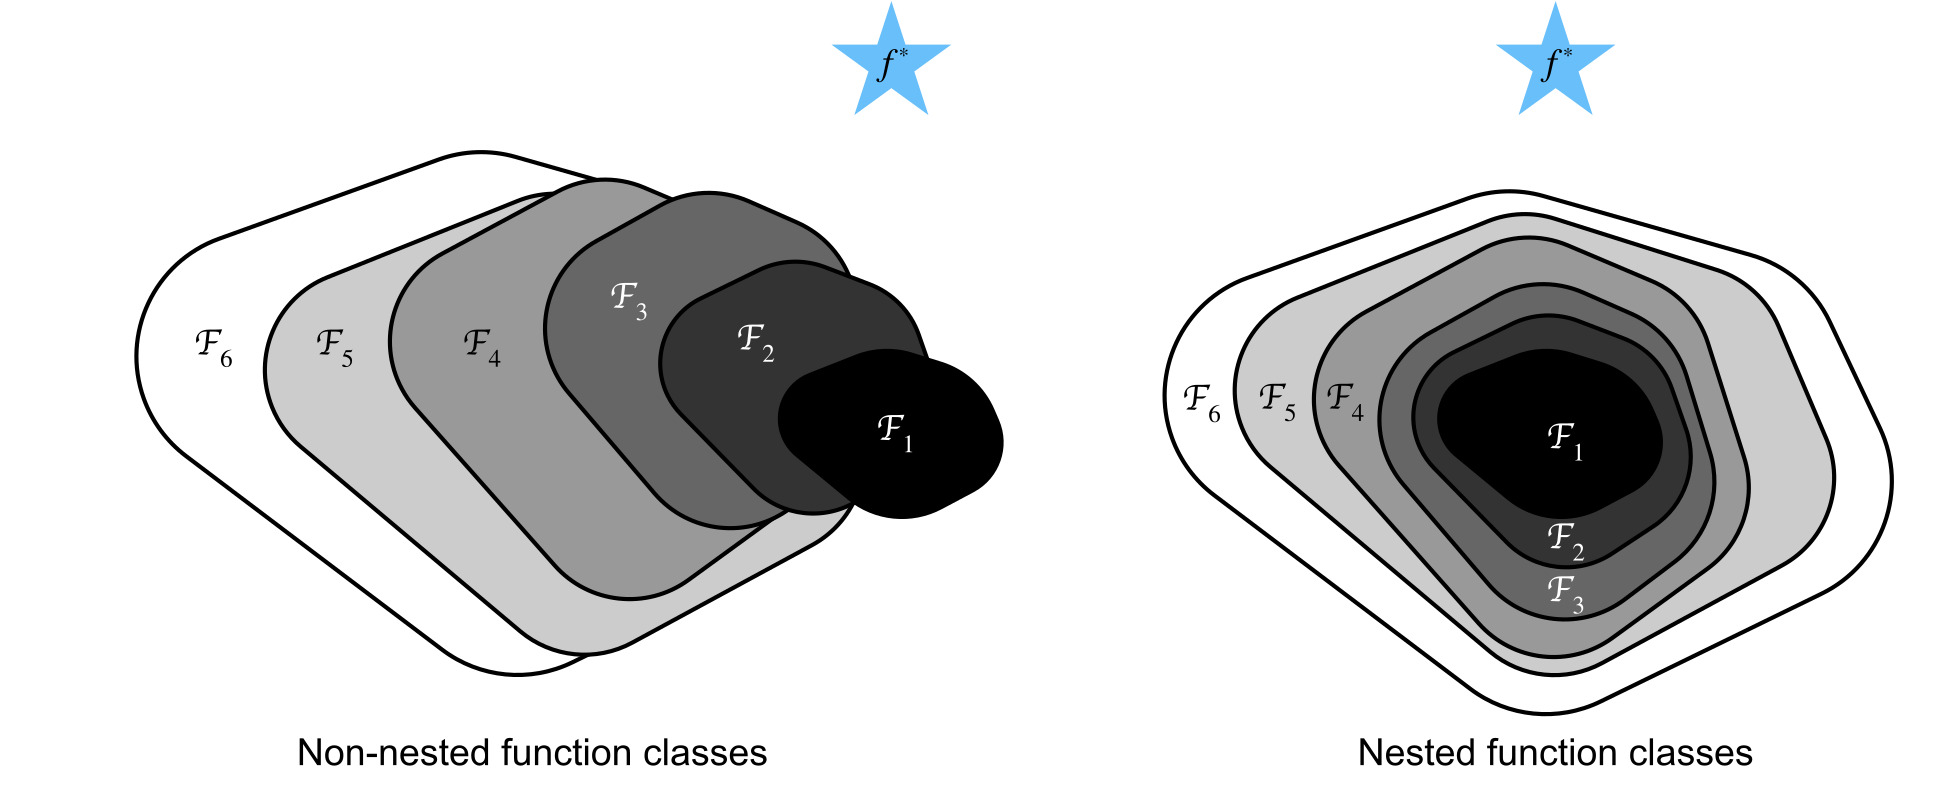
\includegraphics[width=\linewidth, height=3.5cm, keepaspectratio]{Pictures/deep_neural_networks/functionclasses.jpg}
\end{figure}

\begin{enumerate}[itemsep=0.15cm]
    \item Consider $\mathcal{F}$, the class of functions that a specific network architecture (together with learning rates and other hyperparameter settings) can reach

    \item for all $f \in \mathcal{F}$ there exists some set of parameters (e.g., weights and biases) that can be obtained through training on a suitable dataset

    \item assume that $f^\ast$ is the “truth” function that we really would like to find

    \item  it is in $\mathcal{F}$, we are in good shape but typically we will not be quite so lucky.\\
    Instead, we will try to find some $f_\mathcal{F}^\ast$ which is our best bet within $\mathcal{F}$.\\
    For instance, given a dataset with features $\mathbf{X}$ and labels $\mathbf{y}$, we might try finding it by solving the following optimization problem:
    $
        \hfill
        f^*_\mathcal{F} \stackrel{\textrm{def}}{=} \mathop{\mathrm{argmin}}_f L(\mathbf{X}, \mathbf{y}, f) \textrm{ subject to } f \in \mathcal{F}
        \hfill
    $

    \item regularization may control complexity of $\mathcal{F}$ and achieve consistency, so a larger size of training data generally leads to better $f^*_\mathcal{F}$.

    \item It is only reasonable to assume that if we design a different and more powerful architecture $\mathcal{F}'$ we should arrive at a better outcome.\\
    we would expect that $f^*_{\mathcal{F}'}$ is “better” than $f^*_{\mathcal{F}}$.\\
    However, if $\mathcal{F} \not\subseteq \mathcal{F}'$ there is no guarantee that this should even happen.\\
    In fact, $f^*_{\mathcal{F}'}$ might well be worse.
    \begin{enumerate}
        \item for non-nested function classes, a larger function class does not always move closer to the “truth” function $f^*$

        \item though $\mathcal{F}_3$ is closer to $f^*$ than $\mathcal{F}_1$, $\mathcal{F}_6$ moves away and there is no guarantee that further increasing the complexity can reduce the distance from $f^*$

        \item With nested function classes $\mathcal{F}_1 \subseteq \cdots \subseteq \mathcal{F}_6$, we can avoid the aforementioned issue from the non-nested function classes.

    \end{enumerate}

    \item only if larger function classes contain the smaller ones are we guaranteed that increasing them strictly increases the expressive power of the network.

    \item if we can train the newly-added layer into an identity function $f(\mathbf{x}) = \mathbf{x}$, the new model will be as effective as the original model. As the new model may get a better solution to fit the training dataset, the added layer might make it easier to reduce training errors.


\end{enumerate}



\section{Neural Architecture Search (NAS) (2016) \cite{dnn-1}} \label{neural architecture search (NAS)}

\begin{enumerate}
    \item their cost is usually enormous, relying on brute-force search, genetic algorithms, reinforcement learning, or some other form of hyperparameter optimization. 
    
    \item Given a fixed search space, NAS uses a search strategy to automatically select an architecture based on the returned performance estimation.
    
    \item The outcome of NAS is a single network instance.

\end{enumerate}


































